\chapter{Tinjauan Pustaka dan Dasar Teori}

\section{Tinjauan Pustaka}

Lorem ipsum some placeholder text here.


\section{Dasar Teori}

\subsection{Antarmuka Sistem Operasi (\textit{Shell})}

\subsection{Linux, \textit{Unix-like}, dan Standar POSIX}

\subsection{Dukungan Kompatibilitas Linux atau \textit{Unix-like} di Windows Pra-WSL}

Teknologi yang digunakan dalam skripsi ini, Windows Subsystem for Linux, bukan merupakan satu-satunya usaha yang digunakan untuk membawa kompatibilitas Linux atau Unix-like ke dalam lingkungan sistem operasi Windows. Microsoft memiliki sejarah panjang dalam membawa dukungan Linux atau Unix-like ke dalam lingkungan Windows.

Sebelum mengembangkan WSL, Microsoft memiliki sejumlah usaha terdahulu yang bertujuan membawa dukungan Linux/Unix-like ke dalam sistem operasi Windows. Dalam proses pengembangan Windows NT yang saat ini mendasari versi-versi Windows modern (Windows 2000 dan setelahnya), Microsoft mendesain sistem operasi tersebut sedemikian rupa agar bersifat modular dan mendukung berbagai macam "subsistem". Pada awal pengembangannya, Windows NT direncanakan memiliki tiga buah subsistem, yakni subsistem Win32, subsistem OS/2 (untuk mendukung interoperabilitas dengan sistem operasi OS/2 milik IBM), dan subsistem POSIX (untuk mendukung interoperabilitas dengan sistem-sistem berbasis Linux, UNIX, atau Unix-like yang sedang populer di kalangan bisnis pada masa itu). Seiring waktu, Microsoft memutus dukungan dan pengembangan lebih lanjut terhadap subsistem OS/2 karena adanya permasalahan bisnis dengan IBM.

Berbeda dengan subsistem OS/2 yang telah mati, dukungan dan pengembangan terhadap subsistem POSIX masih terus berjalan. Secara umum, terdapat tiga iterasi teknologi subsistem POSIX/UNIX yang dikembangkan oleh Microsoft:

\begin{enumerate}
    \item \textbf{Microsoft POSIX Subsystem.} Teknologi ini merupakan teknologi asli kembangan Microsoft yang ada sejak awal pengembangan Windows NT. Teknologi ini tersedia untuk sistem operasi Windows NT 3.1 hingga Windows 2000.
    \item \textbf{Windows Services for Unix (SFU).} Produk ini sesungguhnya adalah teknologi milik perusahaan bernama PTS yang dilisensikan kepada Microsoft. Produk ini menggantikan Microsoft POSIX Subsystem sejak sistem operasi Windows XP dan Windows Server 2003.
    %Teknologi yang membawahi (...) ini sejatinya merupakan hasil pengembangan
    \item \textbf{Subsystem for Unix-based Applications (SUA).}
    % Teknologi ini sejatinya merupakan pengembangan lebih lanjut dari SFU.
    % Teknologi ini pada awalnya bernama subsistem Interix dan berganti nama setelah Microsoft mengakuisisi perusahaan pengembangnya. Setelah akuisisi, produk ini tidak lagi berdiri sebagai produk terpisah, tetapi menjadi salah satu komponen dari Windows Services for Unix (SFU). Komponen ini tersedia sejak 
\end{enumerate}

% Reason against elaborationg further: The lack of new sources due to the nature of this topic that is "historical information".

% https://link.springer.com/chapter/10.1007/978-1-4842-6038-8_1

Di samping solusi-solusi yang [telah] ditawarkan oleh Microsoft tersebut, terdapat pula beragam solusi-solusi pihak ketiga yang meraih tujuan yang sama. Solusi-solusi pihak ketiga ini ada baik guna mengisi kekosongan dukungan oleh Microsoft secara langsung maupun sebagai substitusi (\textit{substitute}) yang menggantikan solusi bawaan milik/buatan Microsoft karena [mungkin] solusi tersebut dirasa kurang atau masih belum sempurna.

\begin{enumerate}
    \item \textbf{Colinux.}

    \item \textbf{Cygwin.}
\end{enumerate}

\subsection{Windows Subsystem for Linux (WSL)}

Windows Subsystem for Linux merupakan usaha terbaru Microsoft dalam membawa kompatibilitas Unix/Linux ke dalam lingkungan Windows.

\subsection{Dukungan Kompatibilitas Linux atau \textit{Unix-like} di Windows oleh Pihak Ketiga}

Microsoft tidak sendirian dalam mengembangkan dukungan lingkungan Linux atau \textit{Unix-like} ke dalam sistem operasi Windows; terdapat beragam pilihan pihak ketiga yang dapat membawa dukungan lingkungan Linux atau \textit{Unix-like} ke Windows.

\subsection{Teknologi Penampilan Antarmuka Grafis dan Sistem Perjendelaan (\textit{Windowing System}) pada Lingkungan Linux: X11/Xorg dan Wayland}

\subsection{Dukungan Antarmuka Grafis pada Windows Subsystem for Linux: Windows Subsystem for Linux GUI (WSLg)}

Microsoft pertama kali menyatakan dukungan penjalanan perangkat lunak berantarmuka grafis (GUI) di Windows Subsystem for Linux versi 2 (WSL2) secara bawaan (\textit{built-in}) pada perhelatan pengembang tahunan Microsoft Build 2021.

Dalam pengembangan fungsionalitas antarmuka grafis pada Windows Subsystem for Linux, Microsoft berkomitmen untuk mengikuti standar yang telah ada pada lingkungan Linux.

\begin{figure}
    \centering
    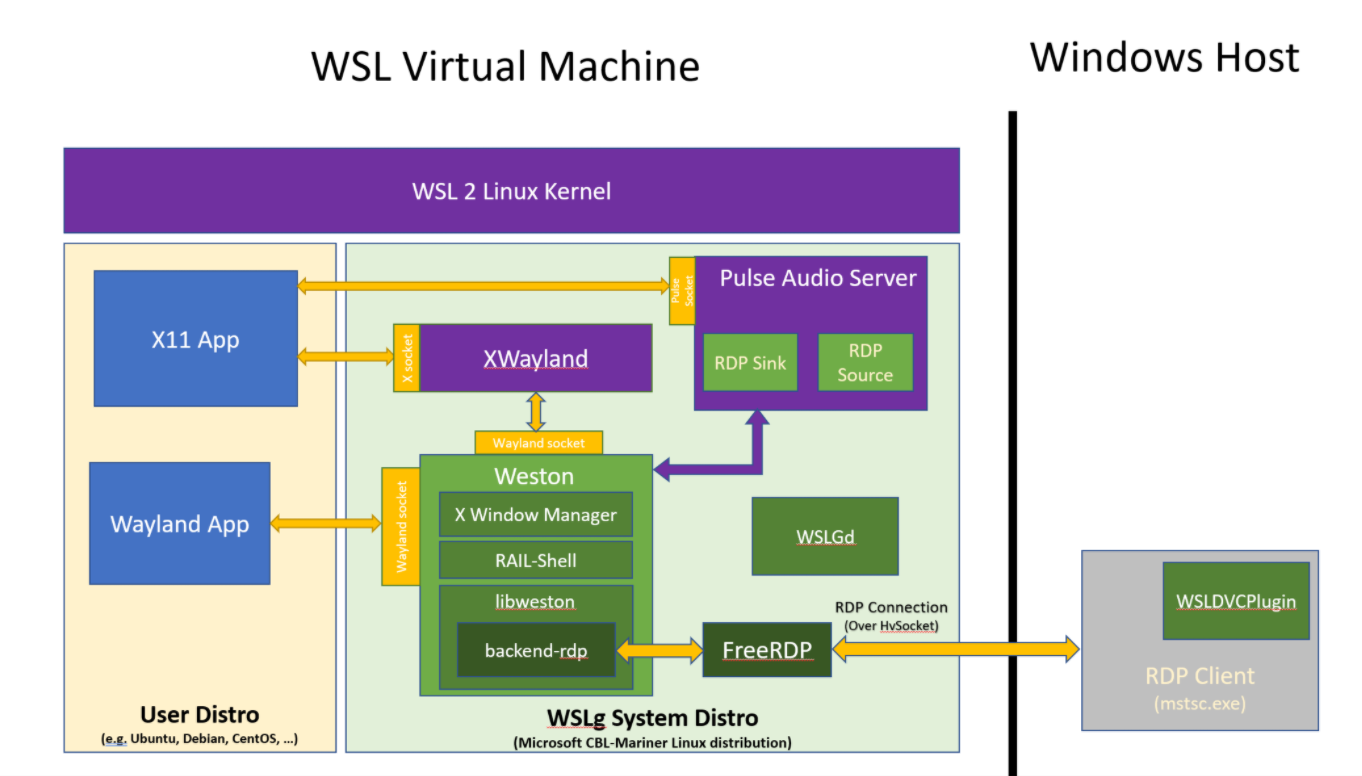
\includegraphics[width=0.5\linewidth]{wslg-architecture.png}
    \caption{Arsitektur Windows Subsystem for Linux GUI (WSLg)}
    \label{fig:enter-label}
\end{figure}

% https://link.springer.com/chapter/10.1007/978-1-4842-6873-5_1
% https://devblogs.microsoft.com/commandline/wslg-architecture/

\subsection{D-Bus}

\subsection{Windows App SDK}

\section{Analisis Perbandingan Metode}

Lorem ipsum.

\section{Pertanyaan Tugas Akhir (Jika Perlu)}

Lorem ipsum.

